\graphicspath{{content/1_literatureReview/figures/}}
\section{Current Sensors}

\subsection{Techniques}
Measurement techniques are usually either "invasive" or "non-invasive". Invasive techniques need to be built into the circuit directly and can have a significant affect
on its operation, whereas non-invasive techniques may be added after the initial circuit design e.g. by measurement of a conductor's magnetic field.
A list of a few of these techniques \cite{currentSenseMethods} include:
\begin{itemize}
    \item A current-sensing resistor in series, which uses Ohm's law with a voltage measurement to calculate current.
    \item Hall element sensors, which measure the potential difference created as a result of the main current's magnetic field bending another current left/right.
    \item Direct coil techniques, which make using of Faraday's law.
\end{itemize}

\begin{figure}[h!]
    \centering
    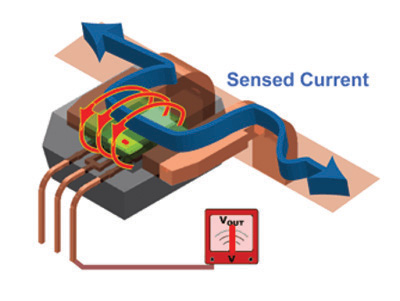
\includegraphics[width=.3\linewidth]{currentSensing_hall_effect}
    \captionof{figure}{Hall Effect Sensor Working Principle \cite{currentSenseHallEffect}}
    \label{fig:hall-effect}
  \end{figure}

\subsection{High-Side vs Low-Side}
This distinction refers to the placement of a current-sense element (e.g. resistor) relative to the load. For circuits which draw higher currents, high-side sensing can be used
(placing the resistor closer to the positive side of the voltage source) and is often more convenient. Low-side sensing, on the other hand, can potentially cause ground loop
issues \cite{currentSenseLowHighSide}, but has the ability to detect faults (e.g. short-circuits) earlier.

\subsection{AC, DC and Power Requirements}
As mentioned, there are various non-invasive and even wireless techniques used to measure current. Coil techniques make use of induction and therefore require AC to operate.
The Hall effect and sense resistors, on the other hand, may be used in the DC case. Wireless techniques have benefits over resistors in that they can be configured to draw much less power,
whereas sense resistors usually require high power handling capabilities as they pass all current drawn by the actual load through them.
